\documentclass{IEEEtran}

\hbadness=999999

% Packages
\usepackage{amsmath}
\usepackage{physics}
\usepackage[cmintegrals]{newtxmath}
\usepackage{graphicx}
\usepackage{xurl} % Makes urls better
\usepackage{fancyhdr}
\usepackage{caption}
\usepackage{circuitikz}
\graphicspath{{./images}}


% Title Stuff
\title{Experiment 2: Single-Phase Transformers}
\author{Chase Lotito, Blake Jourdan, Noah Holland}
\date{}

% Begin document
\begin{document}

\pagestyle{fancy}

\fancyhf{}
\fancyhead[L]{ECE385L: Experiment 2 - Single Phase Transformers}

% Make the title
\maketitle

% ABSTRACT
\begin{abstract}
    % [A brief statement on what you plan to do in this project.]
    The following experiment aquainted us with the single-phase transformer. We observed the transformer while disassembled, noting the geometry of the coil and core. Then, after reassembly, we noted the behavior of the transformer when exciting the primary coil with a sweep of voltages. From this we explain the humming from the transformer, and the results of a open-circuit and short-circuit test.
\end{abstract}

\section{Transformer Humming}

During the experiment, whenever we applied our AC voltage to the primary coil of the transformer, the transformer made a low-pitch humming noise. So, by exciting the device, some of the electrical energy is spent mechanically vibrating it.

The cause is \emph{magnetostriction}, where changing magnetic fields cause particles in a ferromagnetic material to move and change in size \cite{magnetostriction}. Since the particles are continually being excited by the 60Hz source, we get a vibrating magnetic device.

For a DC source, the frequency is zero, so any ferromagnetic particles will move once and reach an equilibrium, so no continual vibrations can cause humming.

\section{Dislodging the Transformer Yoke}

Before performing the open-circuit test on the transformer, we applied an input voltage while the yoke (top of core) was loosened.

% TODO: Explain the magnetic force on Yoke

% Explain current rising in the same test. Is core reluctance increasing or decreasing as we attempt to remove the yoke.

When we rotate the yoke from its normal position, the cross-sectional area that it makes at the corners of the magnetic core decreases. Remembering the formula for reluctance:

\begin{equation}
    \mathcal{R} = \frac{l}{\mu A}
    \label{eq:reluctance}
\end{equation}

Here it's easy to see that a decreasing cross-sectional area \(A\) causes a increase in core reluctance \(\mathcal{R}\).

We also noted that the source current to the transformer increased when we dislodged the yoke, but this is a direct cause of our increasing core reluctance. From the formula for magnetomotive force (mmf):

\begin{equation}
    Ni = \Phi \mathcal{R}
    \label{eq:mmf}
\end{equation}

Since the coil turns and flux are unchanged, we can see that increasing core reluctance will cause increasing coil current as \(i \propto \mathcal{R}\).

\section{Open-Circuit and Short-Circuit Tests}

% Insert collected data.
\smallskip
\begin{center}
\begin{tabular}{ |c|c|c|c| }
    \hline
    Source & Source & Source & Secondary Coil \\
    Voltage (V) & Current (A) & Power (W) & Voltage (V) \\
    \hline
    30 & 0.085 & 0.0 & 65.5 \\
    \hline
    60 & 0.180 & 1.0 & 133.2 \\
    \hline
    90 & 0.290 & 2.1 & 196.7 \\
    \hline
    115 & 0.435 & 5.1 & 251.1 \\
    \hline
    120 & 0.490 & 6.5 & 261.6 \\
    \hline
    125 & 0.500 & 8.3 & 276.5 \\
    \hline
\end{tabular}
\captionof{table}{Open-Circuit Test Data}
\end{center}

\subsection{Magnetic Flux Density and Magnetic Field Intensity of Core}

From Table 3.1, we can calculate the maximum magnetic flux density \(  B_{\text{max}} \) and maximum magnetic field intensity \(H_{\text{max}}\) using the following equations in \cite{labmanual}.

\begin{align}
    B_{\text{max}} &= \frac{\sqrt{2} V_{\text{rms}}}{N_1 A_c \omega} \\
    H_{\text{max}} &= \frac{\sqrt{2} N_1 I_0}{l_{\text{eff}}}
\end{align}

Using the dimensions of the transformer core, we find that \(l_{\text{eff}} = 0.3048 \text{m}\) and \(A_c = 0.00242 \text{m}^2\). On the primary side of the transformer, the number of turns is labelled \(N_1 = 230 \text{T}\). The angular frequency is \(\omega = 2\pi (60 \text{Hz})\). With these values, we get the following table:

% Insert calculated B_max and H_max data.
\begin{center}
\begin{tabular}{ |c|c| }
    \hline
    \(B_{\text{max}}\) & \(H_{\text{max}}\) \\
    \hline
    0.202 & 90.7 \\
    \hline
    0.404 & 192.1 \\
    \hline
    0.607 & 309.5 \\
    \hline
    0.775 & 464.2 \\
    \hline
    0.809 & 522.9  \\
    \hline
    0.842 & 533.6  \\
    \hline
\end{tabular}
\captionof{table}{Calculated Values for \(B_{\text{max}}\) \& \(H_{\text{max}}\) }
\end{center}


\newpage
Plotting this data:

\begin{figure}[h!]
    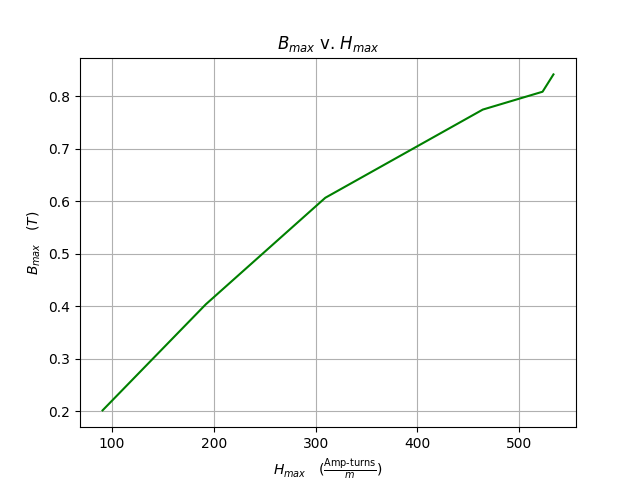
\includegraphics[width=\columnwidth]{bh-plot.png}
    \caption{Magnetization curve for 1\(\phi\) transformer} 
    \label{fig:bh-og}
\end{figure}

Also, plotting the excitation current and excitation voltage, we get Fig. \ref{fig:excitation}:

\begin{figure}[h!]
    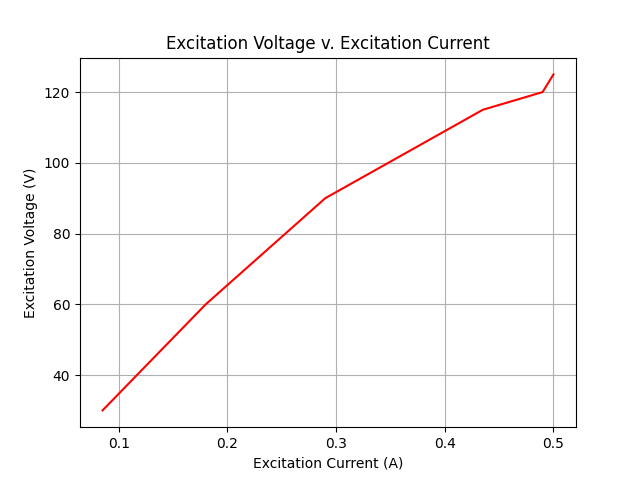
\includegraphics[width=\columnwidth]{vi-plot.png}
    \caption{Excitation Voltage v. Excitation Current}
    \label{fig:excitation}
\end{figure}

As we can see both plots have the exact same curvature, and they're just scaled versions of each other given the equations for \(B_{\text{max}}\) \& \(H_{\text{max}}\). But, we can see both curves saturate as we approach \(120\)V applied to the primary coil. This tells us that as we approach \(120\)V, we start reaching the magnetization limits of the magnetic material that constructs the core of the transformer.

If we reflect Fig. \ref{fig:bh-og} into the third quadrant, and interpolate the data for \(H \in (-H_{\text{max}}, H_{\text{max}})\), we get Fig. \ref{fig:bh-interp}. This plot representing the top half of a completed hystersis loop.

\begin{figure}[h!]
    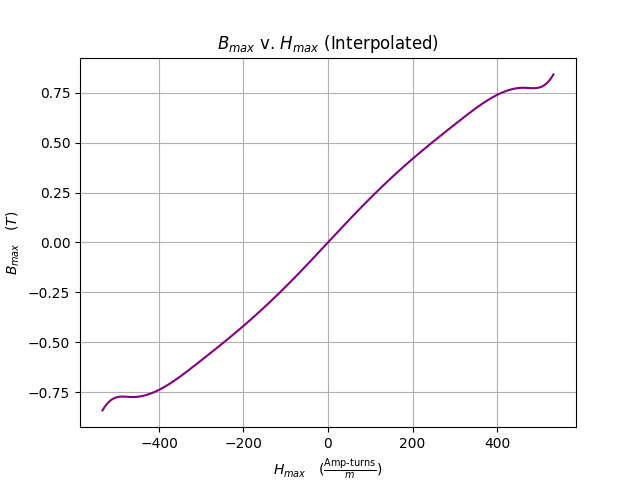
\includegraphics[width=\columnwidth]{bh-interp-plot.png}
    \caption{Interpolated magnetization curve for 1\(\phi\) transformer} 
    \label{fig:bh-interp}
\end{figure}

\subsection{Computation of Magnetizing Branch Elements at \(115\)V}

Using the data from Table 1, we can calculate \(R_c\) and \(X_m\). Since, these are quanities in parallel with the transformer, it is easiest to calculate their reciprocal quanities (conductance \(G\) and susceptance \(B\)) \cite{labmanual}, these are Eq. 5 and Eq. 6.

\begin{align}
    \frac{1}{R_c} &= G_c = \frac{I_{\text{OC}}}{V_{\text{OC}}} \cos {\theta_{\text{OC}}} \\
    \frac{1}{X_m} &= B_m = \frac{I_{\text{OC}}}{V_{\text{OC}}} \sin {\theta_{\text{OC}}}
\end{align}

We need our power factor,

\begin{align*}
    \cos{\theta_{\text{OC}}} &= \frac{5.1 \text{W}}{( 115 \text{V} )( 0.435 \text{A} )} = 0.102
\end{align*}

Which means \( \theta_{\text{OC}} = 84.1^\circ \). Now, we can calculate conductance and susceptance,

\begin{align*}
    G_c &= \frac{0.435}{115} (0.102) = 0.389 \times 10^{-3} \\
    B_m &= \frac{0.435}{115} \sin{84.1^\circ} = 3.76 \times 10^{-3}
\end{align*}

Inverting these to get core resistance and magnetizing reactance,

\begin{align*}
    R_c &= 2572 \Omega \\
    X_m &= 265.8 \Omega
\end{align*}

We also briefly conducted a short-circuit test on the transformer, obtaining the following results,

\begin{align*}
    V_{\text{SC}} &= 4.000 \text{V} \\
    I_{\text{SC}} &= 1.505 \text{A} \\
    P_{\text{SC}} &= 4.000 \text{W} \\
\end{align*}

We can calculate power factor the same as before and get that \( \cos{\theta_{\text{SC}}} = 0.664\), which means \( \theta_{\text{SC}} = 48.4^\circ \). Calculating for the leakage resistance and reactance,

\begin{align}
    R_{\text{eq}} &= \frac{V_{\text{SC}}}{I_{\text{SC}}} \cos {\theta_{\text{SC}}} = 1.76\Omega\\
    X_{\text{eq}} &= \frac{V_{\text{SC}}}{I_{\text{SC}}} \sin {\theta_{\text{SC}}} = 1.99\Omega
\end{align}

So, attributing to copper losses in the transformer, \(Z_{\text{eq}} = 1.76 + j1.99 \Omega\). 

\subsection{Core Reluctance at 115V}

We can calculate the core reluctance at 115V (\(I_1 = 0.435\)A) since, \( N_1I_1 = \Phi \mathcal{R}_c = B A_c \mathcal{R}_c \).

\begin{equation*}
    \mathcal{R}_c = \frac{N_1 I_1}{B A_c} = \frac{(230)(0.435)}{(.775)(0.00242)} = 53.3  \text{k}\frac{\text{A-t}}{\text{Wb}}
\end{equation*}

\subsection{Magnetizing Current v. Excitation Voltage}

Using \(X_m = 265.8 \Omega\), we can calculate the magnetizing current \(I_m\) for \(V_1 = 115, 120, 125 \text{V}_\text{rms}\), since we know that \(I_m = V_1 / X_m\).

\begin{figure}[h!]
    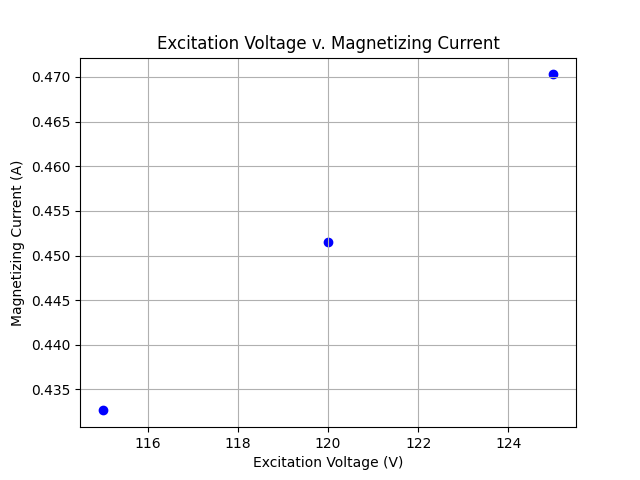
\includegraphics[width=\columnwidth]{mag-current-plot.png}
    \caption{\(I_m\) for 115V, 120V, 125V} 
    \label{fig:mag-current}
\end{figure}

\subsection{Equivalent Circuits}


\begin{figure}[h!]
    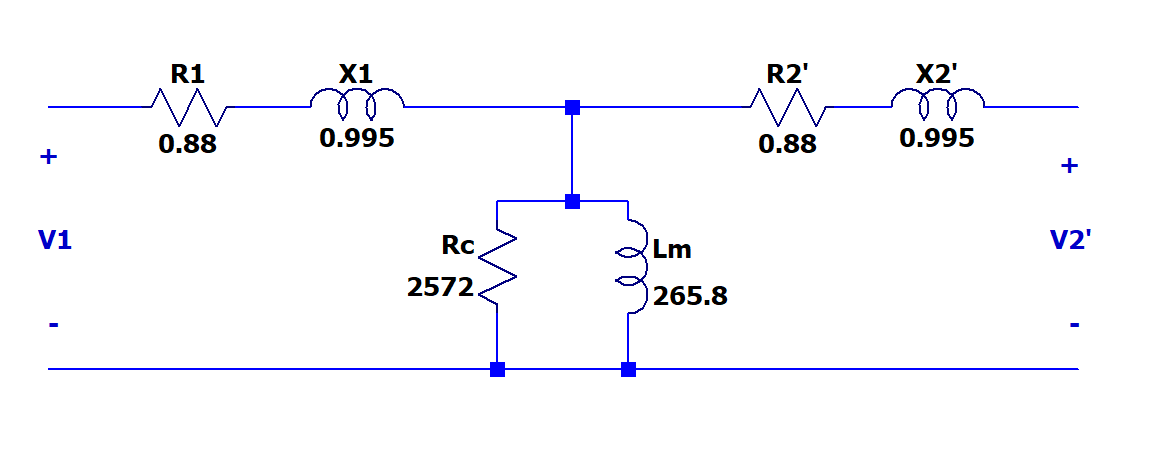
\includegraphics[width=\columnwidth]{eq-ckt.png}
    \caption{Primary Coil Equivalent Circuit} 
    \label{fig:eq-ckt}
\end{figure}

Using the approximation in \cite{labmanual},

 \begin{align*}
    R_1 &= R_2^{'} = 0.88 \Omega \\
    X_1 &= X_2^{'} = j0.995 \Omega 
\end{align*}

\begin{figure}[h!]
    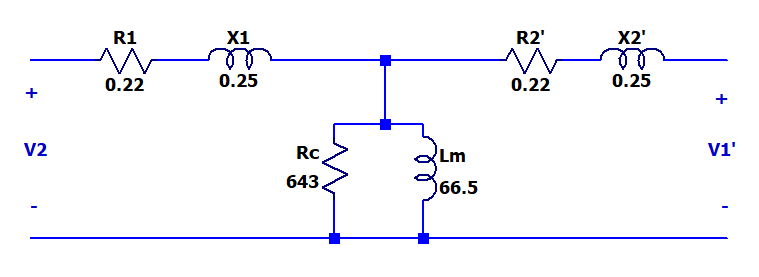
\includegraphics[width=\columnwidth]{eq-ckt-sec.png}
    \caption{Secondary Coil Equivalent Circuit} 
    \label{fig:eq-ckt-sec}
\end{figure}



This gives the transformer equivalent circuit in Fig. \ref{fig:eq-ckt}. Which  only applies for \(V_1 \leq 120\)V as the left side of the circuit is the primary coil, which is the 230 turn side. Similarly, Fig. \ref{fig:eq-ckt-sec} applies for \(V_2 \leq 240\)V as that is the rated voltage for the 460 turns side. 


% REFERENCES!
\bibliographystyle{IEEEtran}
\bibliography{bib.bib}

\end{document}
